\documentclass[12pt]{article}
\input{bayesuvius.sty}
\begin{document}

\begin{figure}[h!]\centering
\begin{minipage}{.5\linewidth}
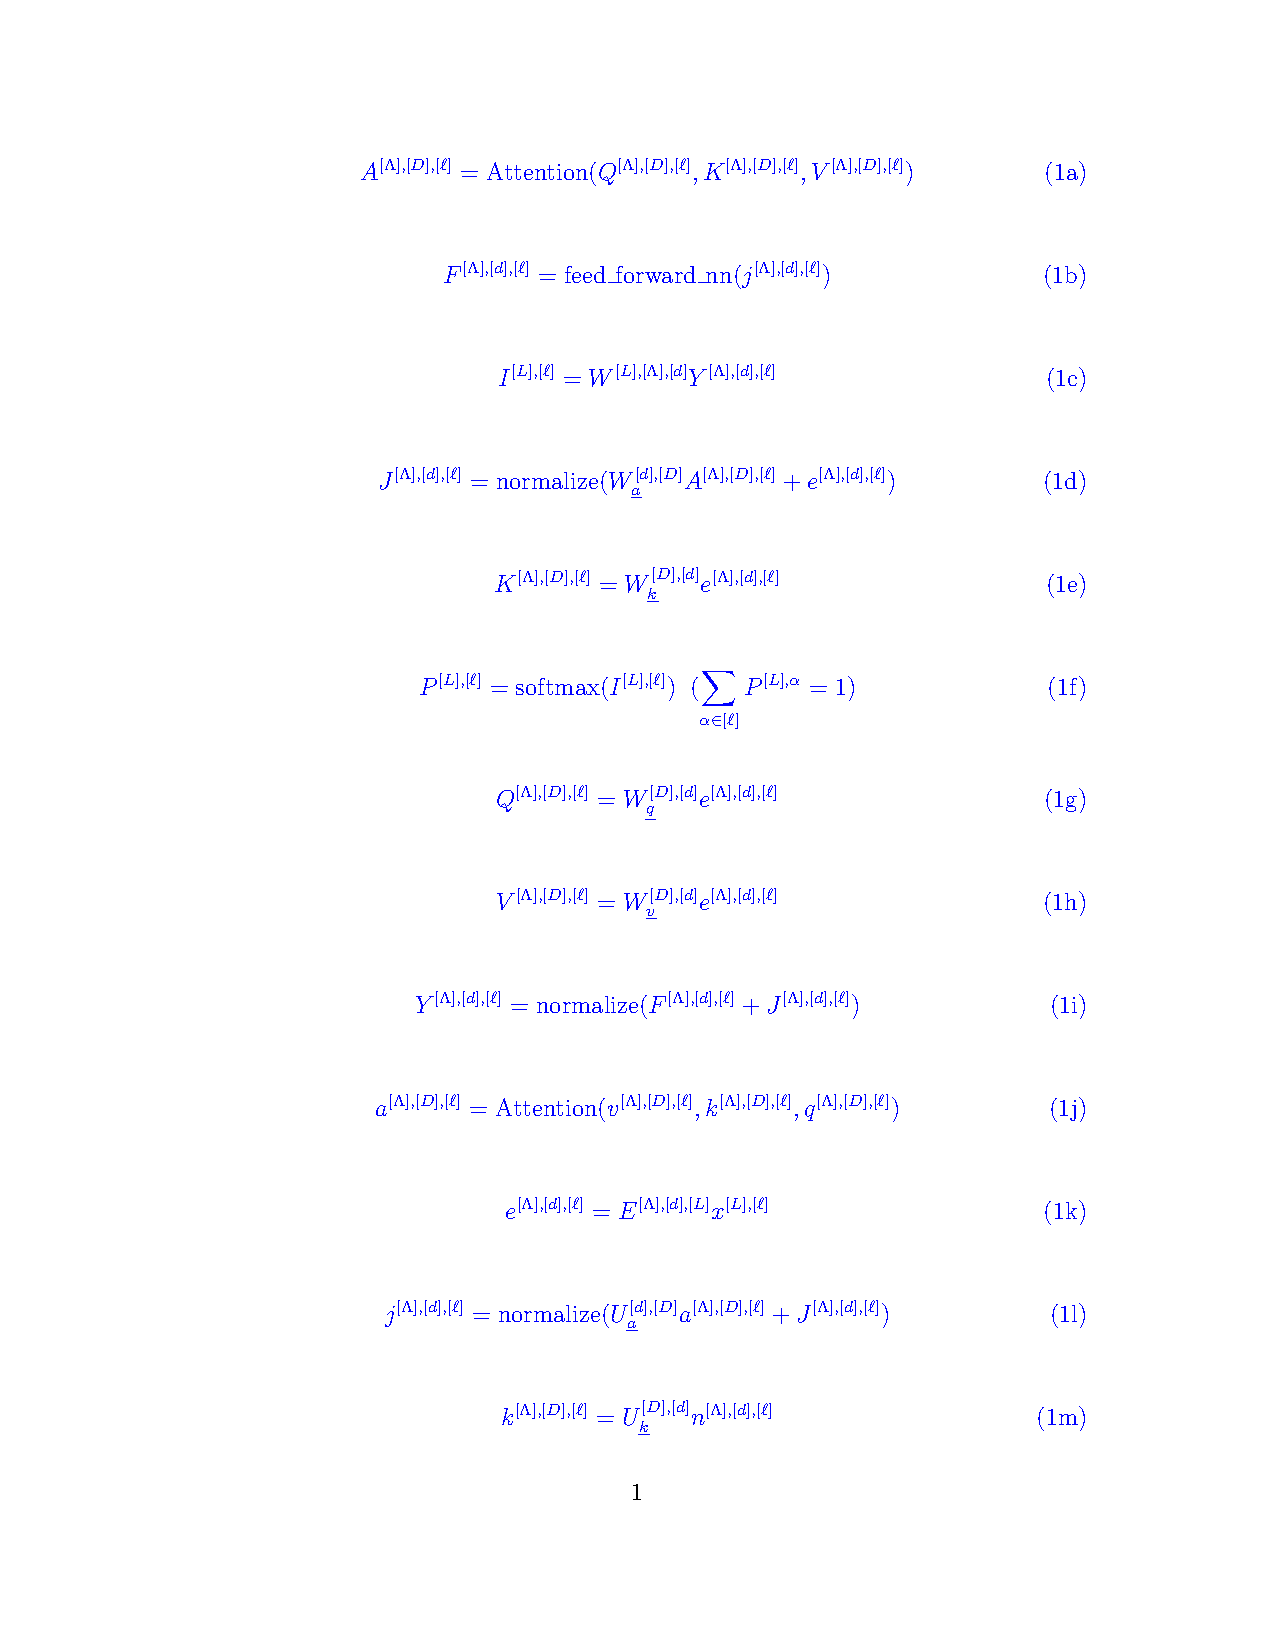
\includegraphics[width=2in]{decoder.jpg}
\end{minipage}%blank lines between minispaces breaks this
\begin{minipage}{.5\linewidth}
$$\xymatrix{
&&&*+[F*:SpringGreen]{\underline{G}^{[D], [L]}}
\\
&&&*+[F*:Orchid]{\underline{I}^{[D], [L]}}\ar[u]
\\
&&&*+[F*:yellow]{\underline{Y}^{[D], [L]}}\ar[u]
\\
&&*+[F*:SkyBlue]{\underline{F}^{[D], [L]}}\ar[ur]&
\\
&&&*+[F*:yellow]{\underline{j}^{[D], [L]}}\ar[uu]\ar[ul]
\\
*+[F*:Dandelion]{\underline{o}^{[L]}}\ar[urrr]&&&
\\
*+[F*:Dandelion]{\underline{q}^{[D], [L]}}\ar[u]&*+[F*:Dandelion]{\underline{k}^{[D], [L]}}\ar[ul]&*+[F*:Dandelion]{\underline{v}^{[D], [L]}}\ar[ull]&*+[F*:yellow]{\underline{a}^{[D], [L]}}\ar[uu]\ar[l]
\\
&*+[F*:Dandelion]{\underline{O}^{[L]}}\ar[urr]&&
\\
*+[F*:Dandelion]{\underline{Q}^{[D], [L]}}\ar[ur]&*+[F*:Dandelion]{\underline{K}^{[D], [L]}}\ar[u]&*+[F*:Dandelion]{\underline{V}^{[D], [L]}}\ar[ul]&
\\
&&&*+[F*:gray]{\underline{p}^{[D], [L]}}\ar[uuu]\ar[ulll]\ar[ull]\ar[ul]
\\
&&&*+[F*:Lavender]{\underline{R}^{[D], [L]}}\ar[u]
}$$
\end{minipage}
\caption{Decoder.}
\label{fig-texnn-for-decoder}
\end{figure}

\begin{subequations}

\begin{equation}\color{blue}
G^{[D], [L]} = I^{[D], [L]}
\label{eq-G-fun-decoder}
\end{equation}

\begin{equation}\color{blue}
I^{[D], [L]} = Y^{[D], [L]}
\label{eq-I-fun-decoder}
\end{equation}

\begin{equation}\color{blue}
Y^{[D], [L]} = {\rm normalize}(F^{[D], [L]} + a^{[D], [L]})
\label{eq-Y-fun-decoder}
\end{equation}

\begin{equation}\color{blue}
F^{[D], [L]} = j^{[D], [L]}
\label{eq-F-fun-decoder}
\end{equation}

\begin{equation}\color{blue}
j^{[D], [L]} = {\rm normalize}(o^{[L]} + a^{[D], [L]})
\label{eq-j-fun-decoder}
\end{equation}

\begin{equation}\color{blue}
o^{[L]} = q^{[D], [L]},k^{[D], [L]},v^{[D], [L]}
\label{eq-o-fun-decoder}
\end{equation}

\begin{equation}\color{blue}
a^{[D], [L]} = {\rm normalize}(O^{[L]} + p^{[D], [L]})
\label{eq-a-fun-decoder}
\end{equation}

\begin{equation}\color{blue}
v^{[D], [L]} = a^{[D], [L]}
\label{eq-v-fun-decoder}
\end{equation}

\begin{equation}\color{blue}
O^{[L]} = Q^{[D], [L]},K^{[D], [L]},V^{[D], [L]}
\label{eq-O-fun-decoder}
\end{equation}

\begin{equation}\color{blue}
Q^{[D], [L]} = p^{[D], [L]}
\label{eq-Q-fun-decoder}
\end{equation}

\begin{equation}\color{blue}
K^{[D], [L]} = p^{[D], [L]}
\label{eq-K-fun-decoder}
\end{equation}

\begin{equation}\color{blue}
V^{[D], [L]} = p^{[D], [L]}
\label{eq-V-fun-decoder}
\end{equation}

\begin{equation}\color{blue}
p^{[D], [L]} = R^{[D], [L]}
\label{eq-p-fun-decoder}
\end{equation}

\begin{equation}\color{blue}
R^{[D], [L]} = 
\label{eq-R-fun-decoder}
\end{equation}

\begin{equation}\color{blue}
q^{[D], [L]} = 
\label{eq-q-fun-decoder}
\end{equation}

\begin{equation}\color{blue}
k^{[D], [L]} = 
\label{eq-k-fun-decoder}
\end{equation}

\end{subequations}


\end{document}  
